%%% Ne pas modifier jusqu'à la ligne 25
\documentclass[a4paper,12pt]{book}
\usepackage[utf8]{inputenc}
\usepackage[french]{babel}
%%\usepackage{CJK}
\usepackage{yhmath}
\usepackage[left=2cm,right=2cm,top=3cm,bottom=2cm, headheight=1.5cm,headsep=1.5cm]{geometry}
%%\usepackage{CJKutf8}
\usepackage{amsfonts}
\usepackage{amsmath,amsfonts,amssymb,dsfont}
\usepackage{graphicx}
\usepackage{enumitem}		%\enumerate-resume
\usepackage[colorlinks=true,unicode={true},hyperindex=false, linkcolor=blue, urlcolor=blue]{hyperref}
\newcommand{\myref}[1]{\ref{#1} page \pageref{#1}}

\addto\captionsfrench{\def\tablename{Tableau}}  %légendes des tableaux
\renewcommand\thesection{\Roman{section}~-~} 
\renewcommand\thesubsection{\Roman{section}.\Alph{subsection}~-~} 
\renewcommand\thesubsubsection{\Roman{section}.\Alph{subsection}.\arabic{subsubsection}~-~} 

\newcommand{\conclusion}[1]{\newline \centerline{\fbox{#1}}}

\setcounter{secnumdepth}{3}
\parindent=0pt

\usepackage{fancyhdr}
\pagestyle{fancy}

\lhead{SJTU-ParisTech} 
%%%%%%%%%%%%%%%%%%%%%%%%%%%%%%%%%%
\chead{DM8}
\rhead{Daniel 518261910024}

\begin{document}
\renewcommand{\labelitemi}{$\blacktriangleright$}
\renewcommand{\labelitemii}{$\bullet$}


\section{Exercice 1 : Datation au carbone 14C}
% \begin{table}[h]
% \begin{center}
%     \begin{tabular}{l|ccccccc}
%     \hline
%                       & $2Ag^+{(aq)}$      & + & $Pb{(s)}$       & = & $2Ag{(s)}$ & + & $Pb^{2+}_{(aq)}$ \\ \hline
%         $c_{initial}$ & $c=5.0*10^{-2}$       &   & $c_{Pb}$      &   & $0$ &  & $0$\\ 
%         $c_{final}$      & $c-2x_v$  &   & $c_{Pb}-x_v$  &   & $2x_v$ & & $x_v$\\ 
%     \end{tabular}
% \end{center}
% \end{table}
Pour la décomposition radioactive du carbone 14, on a sa demi-vie $t_{1/2}=\tau=5730\,ans$. 

En notant $[^{14}C]$ sa concentration, on a $$\frac{1}{2}[^{14}C](t=0)=[^{14}C](t=\tau)=[^{14}C](t=0)\exp(-k\tau)$$, 
d'où $k=\frac{\ln2}{\tau}$. 

Supposons que l'arbre est mort pout le temps $T$, on a donc 
$$
[^{14}C](t=T)=[^{14}C](t=0)\exp(-kT)=74\%[^{14}C](t=0)
$$
d'où $\boxed{T=-\frac{\ln74\%}{k}=-\frac{\ln74\%}{\ln2}\tau}$. 

A.N. $\boxed{T=\frac{\ln74\%}{\ln2}5730=2.5*10^3\,ans}$, l'arbre est mort pour environ $2.5*10^3$ ans.





\section{Mesure de l’énergie d’activation d’une réaction}
% \begin{table}[h]
% \begin{center}
%     \begin{tabular}{l|ccccc}
%     \hline
%                       & $2N_2O_5$      & = & $4NO_2$       & + & $O_2$  \\ \hline
%         %$n_{initial}$ & $n_{1,i}=1.00$       &   & $n_{2,i}=0.300$      &   & $n_{3,i}=0$ \\ 
%         %$n_{final}$      & $n_{1,f}=1.00-6\xi_{eq}$  &   & $n_{2,f}=0.300-\xi_{eq}$  &   & $n_{3,f}=2\xi_{eq}$ \\ 
%     \end{tabular}
% \end{center}
% \end{table}
\subsection{}
Loi d’Arrhenius est la loi empirique: 
$$
\frac{d\ln k}{dT}=\frac{E_a(T)}{RT^2}
$$
avec $k$ la constante de vitesse, $E_a(T)$ l’énergie d’activation de la réaction
\subsection{}
Supposons que l’énergie d’activation $E_a$ est indépendant de $T$, on a donc 
$$
\ln k=-\frac{E_a}{RT}+\ln A
$$
\begin{figure}[h]
    \begin{center}
    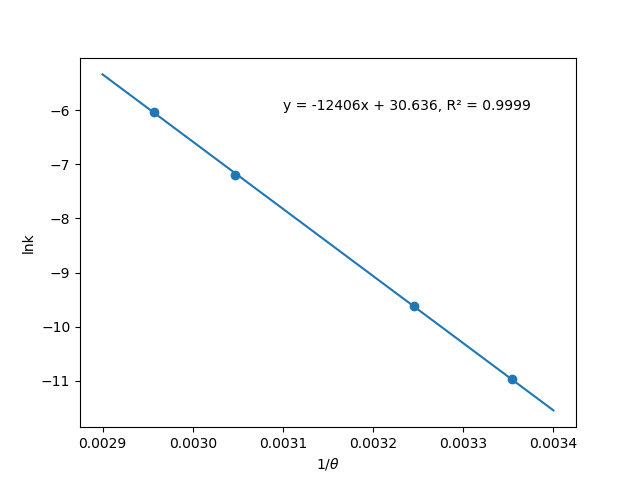
\includegraphics[scale=0.4]{dm8.png}
    \end{center}
    \caption{Ajustement de courbe}
\end{figure}

En effectuant une régression linéaire, on obtient $\boxed{E_a=12406*8.314=103\,kJ\cdot mol^{-1}}$
\subsection{}
On obtient aussi $\ln A=30.636$, d'où $A=2.02*10^{13}\,s^{-1}$
. 

On a donc 
$$\boxed{k=A*\exp(-\frac{E_a}{RT})=2.02*10^13*\exp(-\frac{1.03*10^5}{8.314*303.15})=3.61*10^{-5}\,s^{-1}}$$
 
la constante de vitesse pour $\theta = 30^\circ C$.
\end{document}